
%!TEX root = ../thesis.tex
%*******************************************************************************
%****************************** Third Chapter **********************************
%*******************************************************************************
\chapter{Simulating and Reconstructing SBND}
\label{Chapter6}

% **************************** Define Graphics Path **************************
\ifpdf
    \graphicspath{{Chapter6/Figs/Raster/}{Chapter6/Figs/PDF/}{Chapter6/Figs/}}
\else
    \graphicspath{{Chapter6/Figs/Vector/}{Chapter6/Figs/}}
\fi

%********************************** %Opening  **************************************

Chapter 6 Opening

\newpage

%********************************** %First Section  **************************************
\section{Simulating SBND}

%Modern physics experiments and MC
Many modern physics experiments heavily relies on simulations to develop reconstruction and analysis tools, as well as to understand the physics capabilities of the detector.
Monte Carlo (MC) simulations is the most general and widely used method that use random sampling from a predefined distributions. 
At SBND, the workflow for simulation and reconstruction is provided by the LArSoft framework \cite{}, which has been employed by many other LArTPC experiments.
This framework enables sharing common simulation, reconstruction and analysis tools across collaborations including ArgoNeuT, MicroBooNE, DUNE, SBND and ICARUS.

%Describe the overall workflow
An overview of the simulation workflow is depicted in Fig. \ref{fig:Sim_Workflow}.
The process begins with a generator to produce primary particles that enter the detector, shown by the purple box.
The primary particles can be neutrinos, cosmic muons or BSM particles depending on the type of generator.
The propagation of the primary particle inside and outside the detector, and the resulting energy deposition is simulated using Geant4 \cite{geant4}, shown by the green boxes.
For interactions inside the detector, the charge and light yield is calculated from the energy deposition.
The number of ionisation electrons from charge yield are propagated through the detector to the wire planes using Wirecell tool kit \cite{wirecell}, shown by the red boxes.
The number of scintillation photons from light yield are propagating to the photodetectors using a semi-analytical light library \cite{}, shown by the blue boxes.
For interactions outside of the detector, only the energy depositions within the CRT strips is converted into light yield, shown by the orange box.
The detector response is then simulated for each detector subsystem.
By the end of this stage, the waveforms from each subsystem ideally represent real data.

\begin{figure}[htbp!] 
\centering    
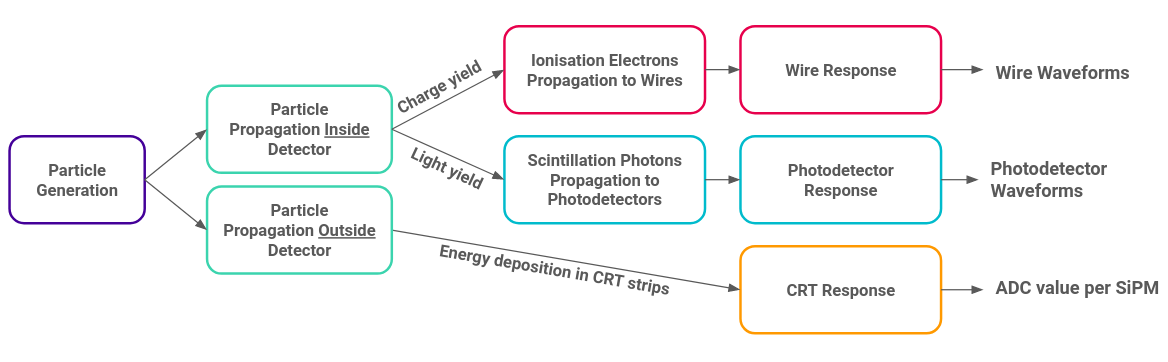
\includegraphics[width=1.0\textwidth]{Sim_Workflow}
\caption[Sim_Workflow]{
Overview of the workflow to simulate the SBND detector.
}
\label{fig:Sim_Workflow}
\end{figure}

The following section covers the simulation workflow for the SBND detector.
Sec. \ref{sec:gen_mevprtl}, \ref{sec:gen_genie} and \ref{sec:gen_corsika} provides the details of the three particle generators to simulate HNLs, neutrinos and cosmic muons respectively.
The simulation of the primary particle propagation using the Geant4 tool kit is outlined in Sec. \ref{sec:gen_g4}.
The propagation of the resulting ionisation electrons and scintillation photons to the respective detection subsystems and their responses are discussed in Sec. \ref{sec:gen_response}. 

%Introduce different types of event generator

\subsection{HNL Generator: MeVPrtl}
\label{sec:gen_mevprtl}

%MeVPrtl Workflow
HNLs are generated using the MeVPrtl generator \cite{}, which is joint effort by ICARUS and SBND collaborators towards a sharing BSM generator.
MeVPrtl was developed as a modular generator, allowing for easy adaptations for different beam sources and detectors, as well as direct interface with the existing LArSoft framework.
The workflow of the MeVPrtl is broken down into 4 stages, as illustrated in Fig. \ref{fig:MeVPrtl_Workflow}.
The generator begins with taking an input of meson fluxes, representing the particles produced from a beam source.
It then simulates the meson decaying to a BSM particle, which is propagated to the detector and decays back into a SM observable.
There are several BSM models already implemented in the MeVPrtl generator, including HNLs, Higgs portal scalars \cite{} and heavy QCD axions \cite{}.


\begin{figure}[htbp!] 
\centering    
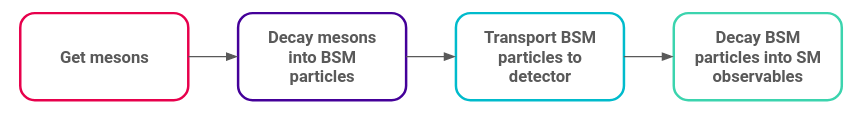
\includegraphics[width=1.0\textwidth]{MeVPrtl_Workflow}
\caption[MeVPrtl_Workflow]{
Overview of the workflow of the MeVPrtl generator.
}
\label{fig:MeVPrtl_Workflow}
\end{figure}

%Each stage validation
For the purpose of generating HNLs coming from the BNB, the generator begins with sampling the charged kaons $K^{+}$ fluxes of the BNB.
Instead of decaying into a SM neutrino, the kaons decay either in-flight or at rest into a HNL, with branching ratio defined by Eq. \ref{eq:kaon_decay_hnl}.
The daughter HNL and lepton are simulated from a two-body decay at rest in the centre of mass frame of the kaon, and then boosted to the parent's lab frame by Lorentz boost.
Due to the HNL having mass, the HNL has less transverse momentum than SM neutrinos and therefore more collimated, travelling preferably to the parent kaon direction.
The Lorentz boost can flip the directions of HNLs from low energy kaons that are originally emitted backwards \cite{DavidePhD}.
The HNL is then propagated to detector by the ray tracing method, which forces the HNL to hit the SBND detector by picking a direction that impinges the particle at the detector front face.
The probability for enforcing the detector intersection is also computed.
Example angular distribution in lab frame of the parent kaons and the HNLs that arrive at the SBND detector is shown in Fig. \ref{fig:kaon_hnl_angle2beam}.
For plotting completeness, the selected parent kaons have energies peaking approximately $0.5\sim1$ GeV, and evenly distributed in the angle with respect to the beam direction, as shown in Fig. \ref{fig:kaon_angle2beam}.
The resulting HNLs of mass 240 MeV and their angles to the beam direction is shown in Fig. \ref{fig:hnl_angle2beam}.
This demonstrates that the acceptance angle of the HNLs to hit the SBND detector is very small ($\theta < 5^\circ$), such that only very forward-going HNLs are most likely to intersect detector.

\begin{figure}[tbp!]
        \centering
        \begin{subfigure}[b]{0.495\textwidth}
            \centering
            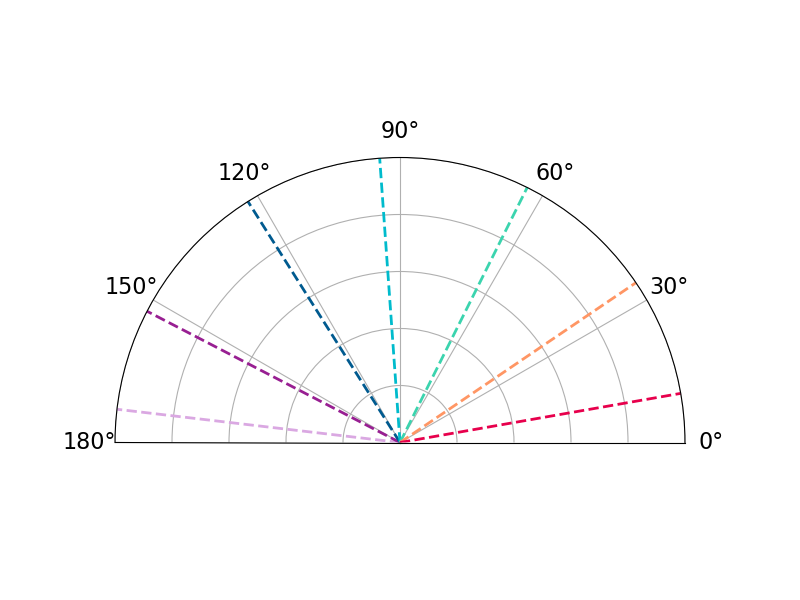
\includegraphics[width=\textwidth]{kaon_angle}
            \caption{Kaons}%
            \label{fig:kaon_angle2beam}
        \end{subfigure}
        \hfill
        \begin{subfigure}[b]{0.495\textwidth}  
            \centering 
            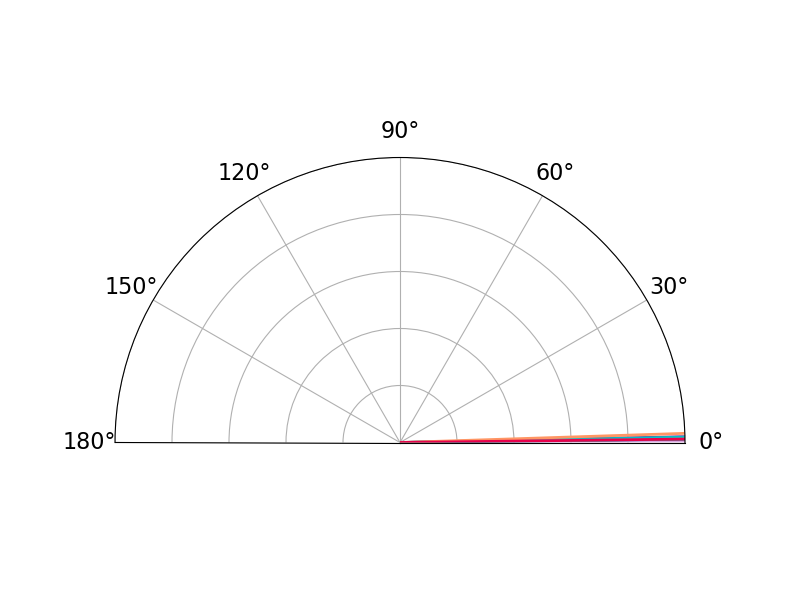
\includegraphics[width=\textwidth]{hnl_angle}
            \caption{HNLs}%
            \label{fig:hnl_angle2beam}
        \end{subfigure}
        \caption[kaon_hnl_angle2beam]{Example distributions of angle to the beam direction, for the parent kaons and for the resulting HNLs that arrive at the detector.}
        \label{fig:kaon_hnl_angle2beam}
\end{figure}

The resulting fluxes of HNL arriving at the SBND detector is depicted in Fig. \ref{fig:HNL_Energy_Spectrum} for the mass range between 140 and 240 MeV.
The fluxes are normalised to the same mixing angle $|U_{\mu4}|^{2} = 1 \times 10^{-7}$ and 3 years of data taking, equivalent to $1 \times 10^{21}$ POT.
At the same mixing angle, the expected HNL rate decreases with lower mass since the branching  ratio of $N \rightarrow \nu\pi^0$ decreases with lower mass, as previously shown in Fig. \ref{fig:branchingRatio}.
Since the $K^{+}$ flux peaks around 0.5 GeV and decreases at higher energy, as previously shown in Fig. \ref{fig:BNB_Meson_Flux}, the HNL fluxes also mainly concentrate in the low energy region, and substantially decrease at higher energy. 
Moreover, across the HNL mass range, there are more energetic HNLs at a lower mass than at a higher mass.
This is due to HNLs coming from a kaon decay and therefore, the lighter the HNL mass, the more kinetic energy is available.
Finally, all the HNL fluxes have a sharp peak near zero, corresponding the HNLs resulting from kaons decay at rest.

Once arrive at the detector, the HNL decays back into the SM observables.
For example of the $\nu\pi^{0}$ final state, the decay width is defined by Eq. \ref{eq:pi0}.
\begin{figure}[tbp!] 
\centering    
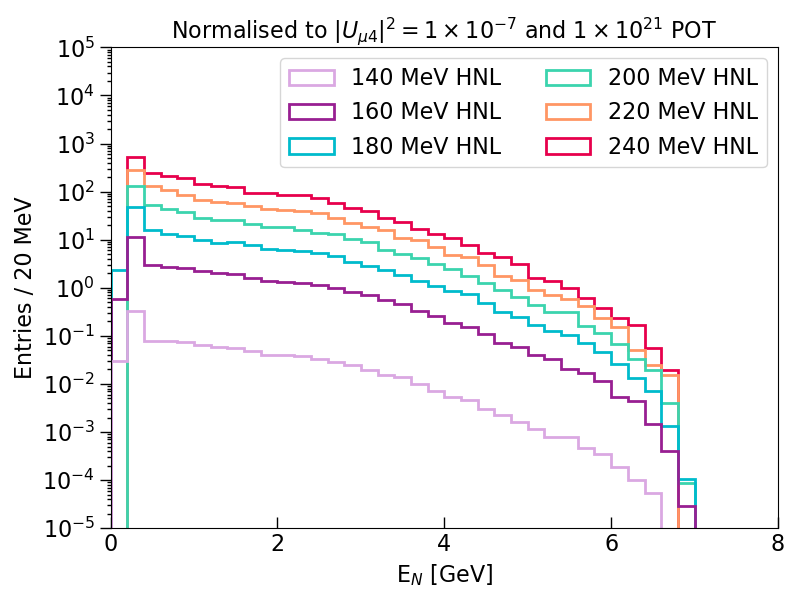
\includegraphics[width=0.65\textwidth]{HNL_Energy_Spectrum}
\caption[HNL_Energy_Spectrum]{
Simulated HNL fluxes for mass ranging from 140 to 240 MeV, normalised to the mixing angle $|U_{\mu4}|^{2} = 1 \times 10^{-7}$ and $1 \times 10^{21}$ POT.
}
\label{fig:HNL_Energy_Spectrum}

%\end{figure}
%\begin{figure}[bp!]

        \centering
        \begin{subfigure}[b]{0.495\textwidth}
            \centering
            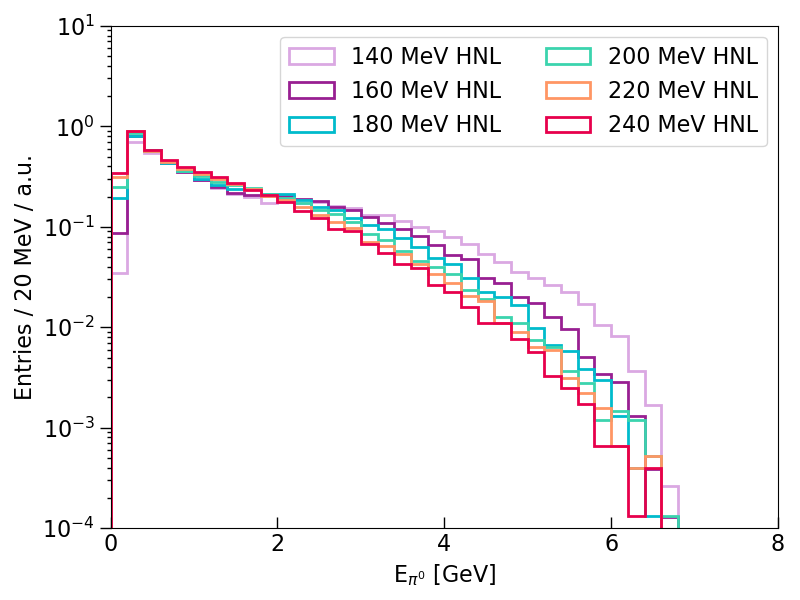
\includegraphics[width=\textwidth]{pi0_energy}
            \caption{Energy Distribution}%
            %\label{fig:kaon_angle2beam}
        \end{subfigure}
        \hfill
        \begin{subfigure}[b]{0.495\textwidth}  
            \centering 
            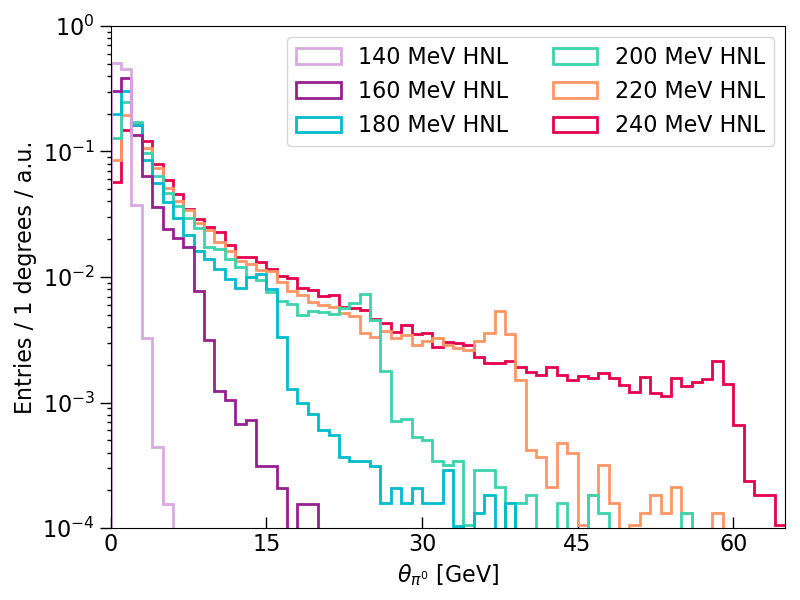
\includegraphics[width=\textwidth]{pi0_angle2Beam}
            \caption{Angle to the Beam Direction Distribution}%
            %\label{fig:hnl_angle2beam}
        \end{subfigure}
        \caption[pi0_distribution]{Kinematic distributions for neutral pions resulting from HNLs decaying inside the SBND detector.}
        \label{fig:pi0_distribution}
\end{figure}
The kinematics of the decay products is simulated for a HNL isotropically decays in its rest frame, and the boosted to its lab frame by Lorentz boost.
Since the parent HNL is very forward-going, the daughter $\pi^0$ is also forward-going, with momenta dependency on the mass of the parent HNL. 
Fig \ref{fig:pi0_distribution} shows the energy and angle to the beam distributions for the daughter $\pi^0$.
The plots are area-normalised for comparison across the mass range of the parent HNL from 140 to 240 MeV. 
The energy distribution of the $\pi^0$ decreases as the HNL mass increases since heavier HNLs are less energetic and therefore, less energy available for the $\pi^0$.
As a result, the angle to the beam of $\pi^0$ also widens with heavier HNL.
Even so, at the HNL mass of 240 MeV, the $\pi^0$ is still collimated with angular distribution dominate in the region $< 30^\circ$. 
Therefore, the di-photon showers from the HNL-originated $\pi^0$ are expected to be more forward-going with respect to the those originate from SM neutrinos.
Finally, the peak in the angular distribution come from low energy HNL resulting from kaons decay at rest.

%Timing
One key motivation of the HNL search is the timing delay between a HNL compared to a SM neutrino, due to a HNL being massive compared to a SM neutrino.
The total time of flight for a HNL or a SM neutrino from the BNB to the SBND detector is illustrated in Fig. \ref{fig:tof_beam_to_detector}.
The first component is the spill time of the protons from the Booster synchrotron, $t_{spill}$, which is the same for both a HNL and a SM neutrino.
The structure of $t_{spill}$ is the beam bucket structure made up of 81 Gaussian buckets with a width of 1.308 ns and a spacing of 19 ns, which was previously detailed in Sec. \ref{sec4BNB}.   

\begin{figure}[htbp!] 
\centering    
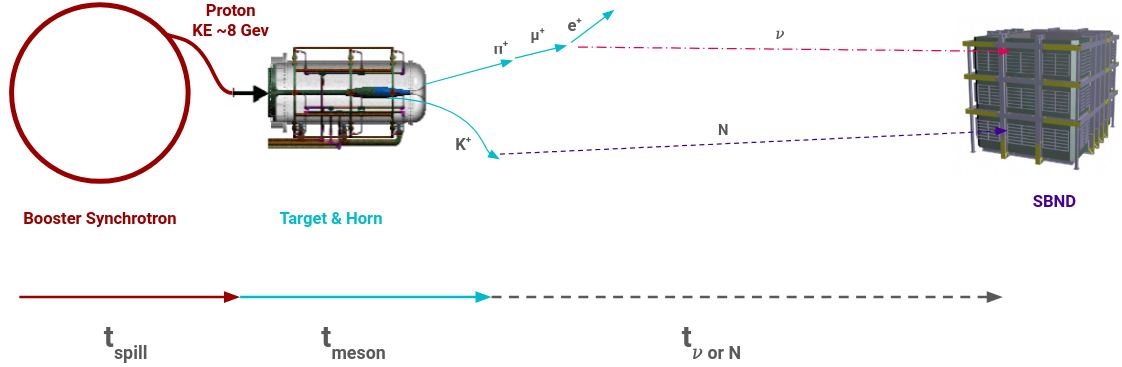
\includegraphics[width=1.0\textwidth]{tof_beam_to_detector}
\caption[tof_beam_to_detector]{
Diagram of the time of flight for a SM neutrino or a HNL, starting from the Booster synchrotron until the interaction time inside the SBND detector.
}
\label{fig:tof_beam_to_detector}
\end{figure}

The second component is the time of the secondary mesons, $t_{meson}$, which is the time from when the mesons are produced until they decay into a HNL or a SM neutrino.
This time accounts for the time the mesons travelling down the decay pipe, and might interact, re-scatter or decay into other mesons.
In the case of the HNL, $t_{meson}$ is primarily the time of flight of the charged kaons $K^+$ before decaying into a HNL.
On the other hands, the SM neutrinos comes from a variety of parent mesons $t_{meson}$, previously listed in Fig. \ref{fig:BNB_neutrino_flux}.
In both cases, $t_{meson}$ introduces some smearing to the nanosecond-bucket structure of $t_{spill}$.

The last component is the time of flight of the SM neutrino or the HNL from the creation point to the interaction point inside the SBND detector.
In the case of the SM neutrinos, since neutrinos are nearly massless, their velocity can be approximated as a speed of light. 
Then, the time of flight of the neutrino is  
\begin{equation}
	t_{\nu} = \frac{d_{\nu}}{c}
\end{equation}
where $d_{\nu}$ is the distance of a neutrino from creation to interaction inside the detector.
Meanwhile, HNLs are massive and therefore, travel at a velocity $v_N < c$.
The time of flight of the HNL is
\begin{equation}
	t_{N} = \frac{d_{N}}{v_N}
\end{equation}
where $d_N$ is the distance of a HNL from creation to decay inside the detector.
Additionally, since the energy of the HNL decreases with its mass, the heavier it is, the slower its velocity.
Thus, heavier HNLs arrive even later compared to lighter HNLs.

The advantage the MeVPrtl generator is the consistency of simulating the time of flight described above, for a HNL using the MeVPrtl generator and for a SM neutrino using the GENIE generator.
Fig. \ref{fig:full_beam} shows the arrival time of the SM neutrinos and 240 MeV HNLs at the front face of the SBND detector, recovering the beam spill structure of the BNB.
The plot is area-normalised to enable the comparison between the two particles. 
Since the SM neutrinos travel nearly at the speed of light, less smearing is introduced and the timing distribution shows sharp Gaussian peaks.
\begin{figure}[bp!] 
\centering    
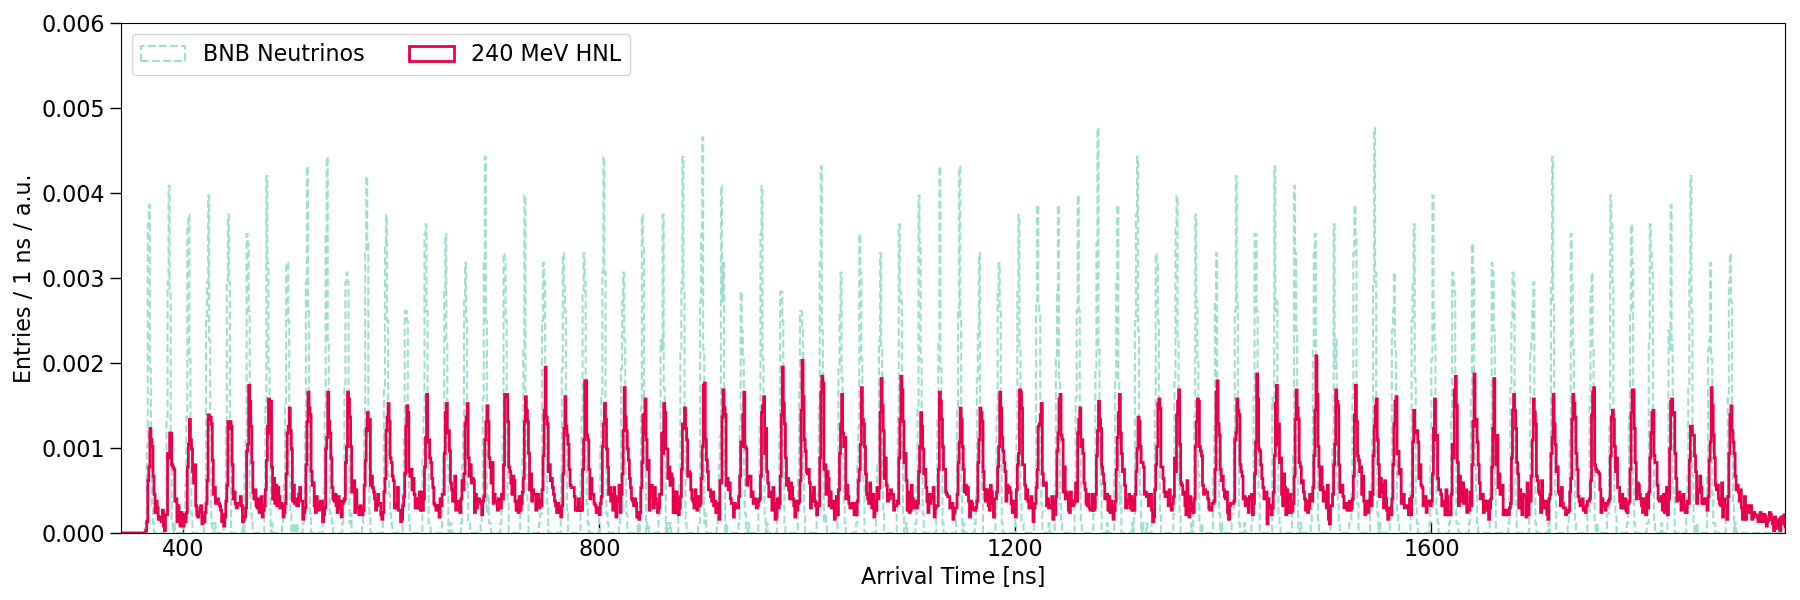
\includegraphics[width=1.0\textwidth]{full_beam}
\caption[full_beam]{
Distribution of the arrival time at the front face of the SBND detector for SM neutrinos simulated by the GENIE generator and for HNLs simulated by the MeVPrtl. 
}
\label{fig:full_beam}
\end{figure}
On the other hands, the HNLs travel slower and therefore, add additional smearing and delay tails to the Gaussian peaks.
For clarity, 81 Gaussian peaks are overlay into one by taking the modulus of 19 ns, as shown in Fig. \ref{fig:beam_modulus}.
The timing distribution of the HNLs show a clear distinction to the SM neutrinos, where delay tails on either sides of the Gaussian peak can be seen.
Across the mass range of HNL from 140 to 240 MeV, the delay tails however do not increase significantly with mass. 

\begin{figure}[htbp!] 
\centering    
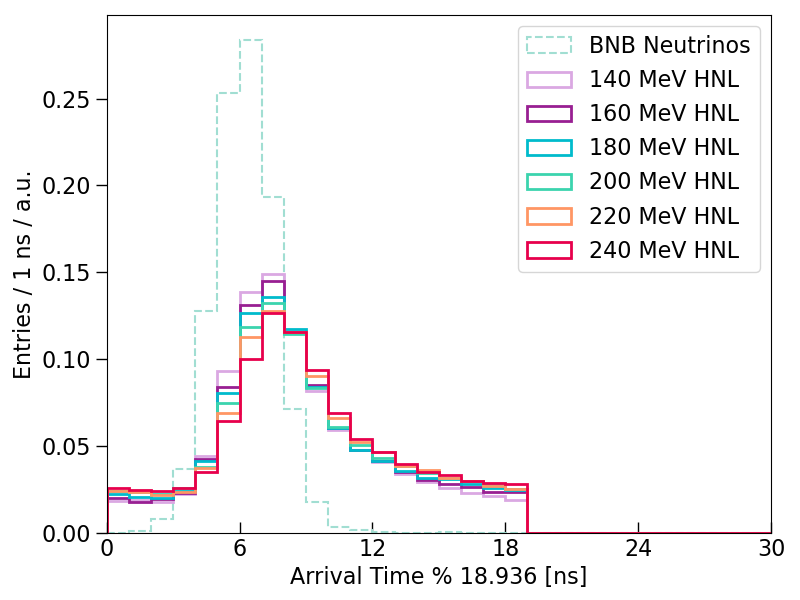
\includegraphics[width=0.65\textwidth]{beam_modulus}
\caption[beam_modulus]{
Modulus of the of arrival time distribution of SM neutrinos and HNLs with mass ranging from 140 to 240 MeV. 
}
\label{fig:beam_modulus}
\end{figure}

\subsection{Neutrino Generator: GENIE}
\label{sec:gen_genie}

%Overview of GENIE

%What kind of tune are being used

SM neutrino interactions are generated by the GENIE generator \cite{genie}, which provides a selection of theoretical and empirical models for different physic process.
These models can be combined into a \textit{tune} by comparing predictions to data from neutrino and electron scattering experiments.
The SBND collaboration is planning to use a tune that was specifically developed to serve as a baseline model for the SBN and DUNE oscillation analysis.
Details for the basis of the tune can be found in Table 1 in Ref. \cite{genie_tune}, with ongoing developments on the choice of models documented in Ref. \cite{genie_tune_github}.  

In general, GENIE first selects a nuclear model that describes the momenta and potential energy of the nucleons to model nuclear effects.
Then, the neutrino flux and the integrated cross section model are used to compute the probability if a neutrino interaction occurs.
The differential cross section is then used to determine the type of neutrino interaction and the kinematic range.
The neutrino interaction types include Quasi-Elastic (QE), Baryonic Resonant Scattering (RES), Coherent Scattering (COH), Deep Inelastic Scattering and $\nu$-e elastic scattering.
DIS interaction can additionally produce hadrons within the nuclei, of which these hadrons can propagate through the nucleus and modify the observed kinematics.
Thus, the choice of Final State Interaction (FSI) model is also crucially important for predicting the observable topology of neutrino interactions since argon is a heavy nuclear target.

In addition to the tune, the GENIE generator also provides a re-weighting scheme to evaluate the systematic uncertainties for a model chosen in the tune.
Due to the scarcity of neutrino interaction data, particularly for $\nu-Ar$ interaction, the uncertainties in cross section modelling tend to be large, and can hamper the capabilities of the HNL sensitivity.  
The neutrino interaction re-weighting scheme, and the resulting systematics uncertainties impact on the HNL search will be discussed in details in Sec. \ref{}.


GENIE simulates neutrino interactions occurring both inside and outside of the detector volume, with boundary defined in Fig. \ref{fig:Rockbox_Volume}.  
All interactions occurring inside the detector volume are strictly kept.
Outside of the detector, a buffer volume is defined as 5 m surrounding the detector volume.
An additional Rockbox volume is defined by extending the buffer volume backwards in the beam direction ($z$-axis) up to 15 m in front of the buffer volume.
Both these volumes are referred to together as the \textit{Rockbox} volume in this thesis.
Neutrino interactions within this volume are kept, whose products can potentially deposit energy in the detector.
These interactions are referred to as \textit{dirt} neutrinos, and constitute to a significant background to the HNL search.
The background rejection of dirt neutrinos will be covered in Sec. \ref{}.

\begin{figure}[htbp!] 
\centering    
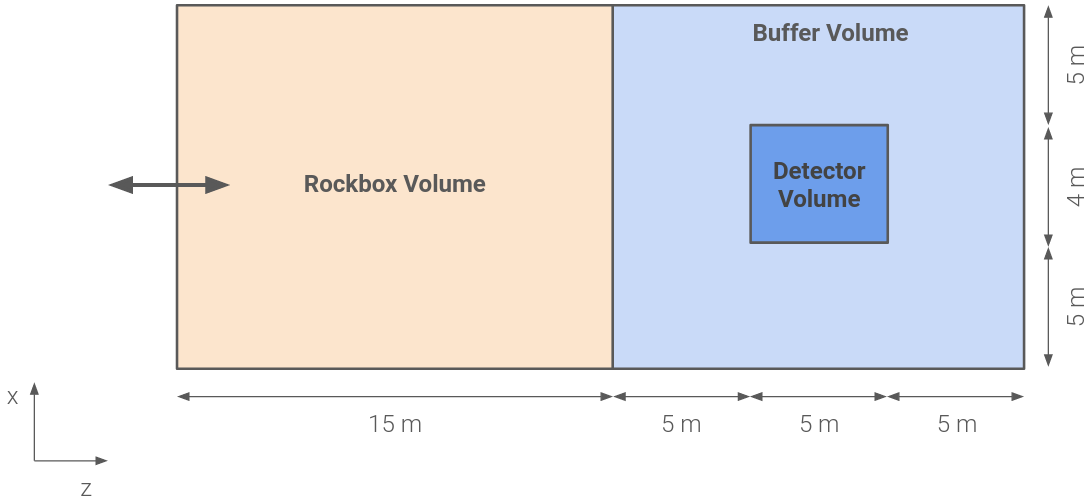
\includegraphics[width=0.85\textwidth]{Rockbox_Volume}
\caption[Rockbox_Volume]{
Diagram showing the volume boundary defined by the GENIE generator to simulate neutrino interactions occurring inside and outside of the detector volume. 
}
\label{fig:Rockbox_Volume}
\end{figure}

\subsection{Cosmic Generator: CORSIKA}
\label{sec:gen_corsika}

%how corsika generator works
Cosmic interactions are simulated using the CORSIKA generator \cite{corsika}.
The generation begins with generating high energy primary particles incident in the Earth's atmosphere, of which only primary protons are kept due to better agreement with MicroBooNE data \cite{}. 
The primaries are then propagated through the atmosphere, interacting with the air to produce secondary decays until reaching the Earth's surface.
Within the SBND simulation workflow, this surface is specified to be just above the roof of the detector building.
The surviving particles are then propagated to the SBND detector.

%Why cosmic simulation is important
From a triggering perspective, there are two types of comic muons as follows 
\begin{itemize}
	\item\textbf{In-time} cosmic muon crosses the detector at the same as a neutrino is present inside the detector, such that the muon is \textit{inside} the beam spill window. The cosmic muon then produces enough light to induce a beam trigger similar to a neutrino.
	\item\textbf{Out-of-time} cosmic muons occurs regardless of the trigger conditions. The muon crosses the detector \textit{outside} the beam spill window, but within the readout window.
\end{itemize}
However, triggering is currently not being simulated in the workflow. 
Only timing requirement is simulated to keep only cosmic muons occurring within the readout window.
Therefore, the simulation does not accurately reflect the cosmic rate once factoring triggering conditions and comparison to data is necessary. 

Being a surface level detector, it is vitally important to understand the cosmic background at SBND due to the exposure to a high cosmic rate.
Once SBND is operational, a particularly useful measurement is the rate of cosmic muons that would cause a beam trigger, however, in absence of the beam.
This is equivalent to measure the rate of cosmic muons that produce sufficient energy inside the detector to mimic a neutrino interaction.
This measurement allows for validation against the CORSIKA generator sampling of the cosmic topology and kinematic distribution. 
Moreover, it also provides an expected cosmic rate given a triggering condition, which can be subsequently added in the simulation workflow to better constrain the cosmic background.

\subsection{Particle Propagation Simulation}
\label{sec:gen_g4}

Once a particle is simulated inside the detector, it is propagated through the detector using the Geant4 tool kit \cite{geant4}.
Geant4 propagates the particle by each step $dx$, where the step length is randomised and capped at 0.3 mm (one order of magnitude less than the wire pitch).
At each step, physics processes are applied to the particle, such as energy deposition, interaction, decay and so on.
The step propagation also accounts for the electric field distortion due to space charge effects, given that the SBND detector is overground and has a high exposure to cosmic.

The main physics process is energy deposition in the detector is ionisation by charged particles.
Similarly to the theory detailed in Sec. \ref{sec3:creation}, the Geant4 tool kit simulates the ionisation process following the Bethe-Bloch formalism tuned to data \cite{geant4_ions}.
The number of ionisation electrons and scintillation photons from the deposited energy are computed using the ModBox recombination model with ArgoNeuT parameters \cite{argoneut_recomb}, and the charge-light anti-correlation from Eq. \ref{eq:Q} and \ref{eq:L}. 
Further discussion about the simulation of recombination, and the impacts of delta ray fluctuations on recombination will be detailed in Sec. \ref{sec7:delta}.
The result from the Geant4 tool kit is a complete set of charge and light yield along the primary particle trajectories through the detector, and the hierarchy of the daughter particles produced from the primary.
The propagation of the charge and light yield to the corresponding detection subsystem are then simulated, to be covered in the upcoming section.

\subsection{Detector Response Simulation}
\label{sec:gen_response}

\subsubsection{Wire Response}

The simulation of the ionisation electrons drifting to the wire planes are done by the WireCell tool kit \cite{wirecell}.
The simulation transports the electrons, and introduces smearing due to detector effects for transporting electrons though liquid argon under an electric field, which is previously discussed in Sec. \ref{sec:edrift}.
This includes charge attenuation due to impurities, smearing of the electron deposition in timing and spatial dimensions due to longitudinal diffusion, transverse diffusion and space charge effect combined.

Once the electrons arrive at the wire plane, a convolution of the field response and the electronic response is performed.
The field response describes the current induced on wires due to ionisation electrons drifting past the induction planes.
Meanwhile the electronic response describes amplification and shaping by pre-amplifiers of wires.
The response functions are in 2-dimensions, one dimension is in time and the other is in wire.
This is to account for long range charge induction effects on wire signal shapes.
A digitisation step is then applied to produce ADC-level, time-domain waveform for each wire channel.
The waveform is parameterised by the ADC resolution, voltage range and baseline specification of the wire readouts. 
Finally, inherent electronics noise is added to the waveform to better match to observed data.
The output simulated waveforms at this stage ideally represent real data waveforms record by the wire readouts, therefore from this point onwards, Monte Carlo and data waveforms should.

\subsubsection{PDS Response}

The simulation of the scintillation photons to the optical detectors, including the transport effects previously detailed in Sec. \ref{sec:photonprop}, are simulated using a combination of semi-analytical model described in Ref. \cite{}, and optical library model available in LArSoft \cite{}.
The choice of which model to use depends on the location of the photon production.
The semi-analytical model is used for those produced inside the active volume of the SBND detector, whilst the optical library model is used to those originate outside of this volume.

The semi-analytical model calculates on-the-flight the geometrical aperture for each optical detector to a scintillation point, given that emission of scintillation photons is isotropic.
The model also extends to not only the direct light component (visible photons), but also the reflected component (VUV photons). 
Corrections for photon transport effects, including Rayleigh scattering and boundary effects, are then applied, to compute the number of photons detected by an optical detector.

However, the semi-analytical method is limited by the geometrical information and do not include scintillation  points outside of the active volume, for example, cosmic tracks crossing behind an optical detector can produce non-negligible light constituting a trigger.
Since the PMTs are the primary subsystems for triggering, it is vital to consider the second order contribution of light produced outside of the active volume for triggering efficiency studies.
The optical library stores a information of the fraction of incident photons for each optical detector for a given scintillation location, which can be looked up for any detector-location pairs during regular simulation. 

For each type of optical detectors, PMTs and X-ARAPUCAs , a respective photon detection efficiency is applied to the number of detected photons.
Then, signal amplification and digitization are simulated, converting photon into an output signal known as single electron response.
Signal shaping such as overshoot and undershoot due to the circuit of the detectors are also simulated.
Finally, random fluctuation in the signal integral and non-linearity response at high light intensities are applied to better mimic data.
The final output is simulated optical waveforms for each type of optical detector, ideally the same as data. 

\subsubsection{Cosmic Ray Tagger Response}

The energy deposition outside of the cryostat from the Geant4 simulation stage is considered for simulating the CRT's response.
For the deposits that cross the CRT strips, the energy into light yield within a strip.
The collection efficiency per SiPM is accounted for by dividing the light yield between the fibres on either side of the strip, based on the lateral position of the energy deposition within the strip. 
The time of the hit is estimated using the time of the energy deposition, accounting for signal attenuation and light propagation delay down the strip towards the SiPM.
Finally, the electronic response is simulated for the CRT readout, by assessing if a pair of SiPMs within a strip goes above a threshold within a pre-defined coincidence window.
The output is a single ADC value per SiPM, where 32 SiPMs per CRT readout are readout simultaneously. 

%********************************** %First Section  **************************************

\section{Reconstructing SBND: TPC Subsystem}
\label{sec:reco_tpc}
%Describe the overall workflow
The output raw data from each detection requires a dedicated reconstruction workflow, as illustrated in Fig. \ref{fig:Reco_Workflow}.
The raw wire waveforms go through the process of signal processing performed by the Wirecell tool kit \cite{wirecell}, followed by a hit finding algorithm to identify hits on the waveform.
The output hits are then used by the Pandora package \cite{pandora} to 3D reconstruct an interaction, denoted as a \textit{slice}.
The raw PDS waveforms also require a similar process of waveform deconvolution, followed by hit finding and reconstruction, outputting reconstructed light-objects denoted as \textit{flash}.
The reconstruction for the CRTs is much simpler compared to other two subsystems, consisting of only a hit finding and a reconstruction step. 
The following Sec. \ref{sec:reco_tpc} will provide the details of the TPC reconstruction workflow from start to end.
Meanwhile, the reconstruction of the PDS and CRT subsystem will be summarised in the next Sec. \ref{sec:reco_others}.

\begin{figure}[htbp!] 
\centering    
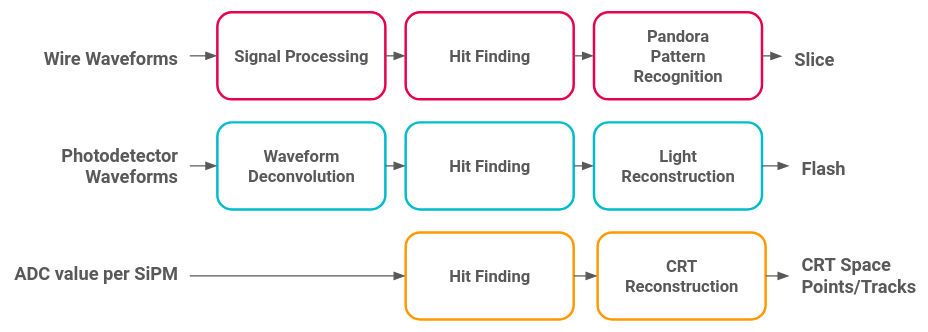
\includegraphics[width=1.0\textwidth]{Reco_Workflow}
\caption[Reco_Workflow]{
Overview of the reconstruction workflow for each detection subsystem of SBND.
}
\label{fig:Reco_Workflow}
\end{figure}

\subsection{TPC Signal Processing}
%Signal Processing
Signal processing is the first crucial step of TPC reconstruction, which is to deconvolve digitised raw waveforms and remove detector effects such as noise, electronics response and field response. 
At SBND, signal processing is implemented using the WireCell tool kit \cite{wirecell}.
The tool has been used by other various LArTPC experiments such as MicroBooNE and ProtoDUNE and has demonstrated the excellent performance to acquire deconvolved charge by performing deconvolution in time and wire dimension over the traditional deconvolution in time dimension only. 

Fig. \ref{fig:signal_processing_steps} \cite{} demonstrates the step by step of the signal processing.
In grey is the true charge deposition on a wire, and in red is the corresponding raw waveform containing signal convolved with noise, electronics response, field response and noise.
The first step in the chain is noise filtering to remove the excess and correlated noise from raw waveforms.
Then, the measured charge is deconvolved from the electronics and field response to recover the original charge deposited on the wire, as shown in orange.
The deconvolution is 2D, where response functions consider the time response of a single wire as well as responses of neighbouring wires.
This step is particularly important for the induction planes to convert bipolar into unipolar signals, such that the integral of the waveform can be used for charge estimation.
\begin{figure}[tbp!] 
\centering    
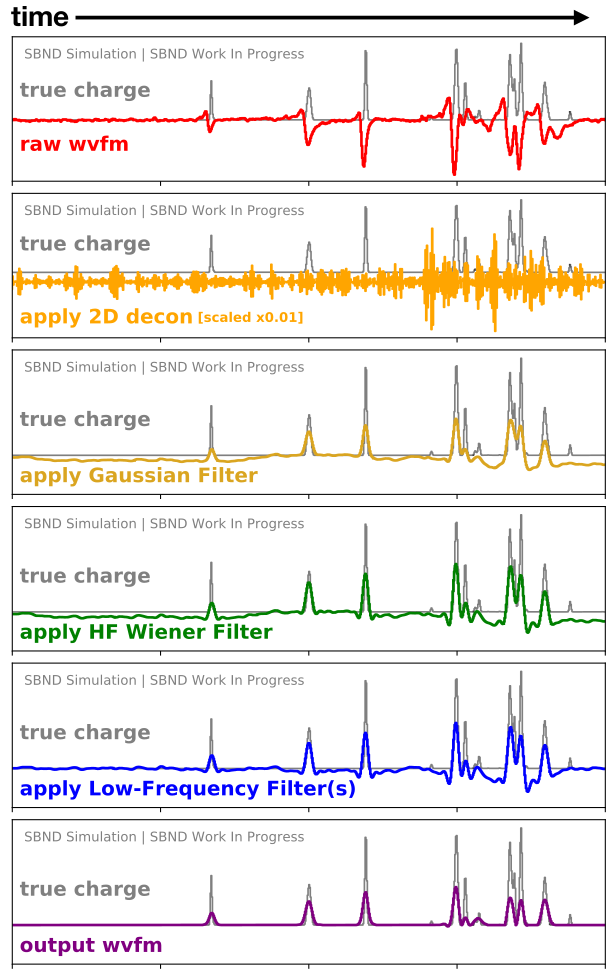
\includegraphics[width=0.45\textwidth]{signal_processing_steps}
\caption[signal_processing_steps]{
Example demonstrating the steps of signal processing applied to a bipolar raw waveform to acquire the final deconvolved waveform.
Fig. from Ref. \cite{}.
}
\label{fig:signal_processing_steps}
%\end{figure}
%\begin{figure}[htbp!] 
\centering    
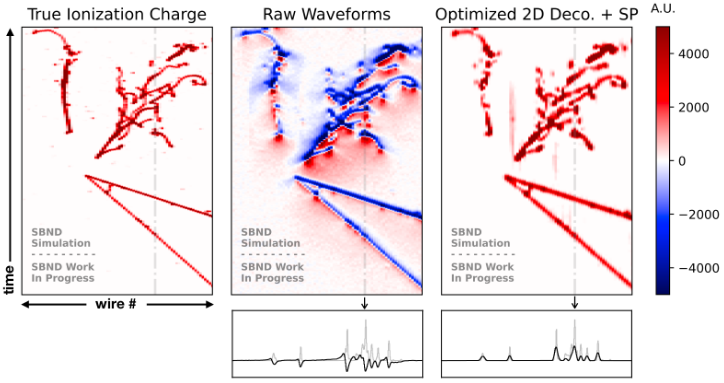
\includegraphics[width=0.75\textwidth]{signal_processing_waveform}
\caption[signal_processing_waveform]{
Event display of a simulated neutrino event using the true ionisation charge (left), raw waveforms (middle) and deconvolved waveforms (right).
Fig. from Ref. \cite{}.
}
\label{fig:signal_processing_waveform}
\end{figure}
Filter functions are applied subsequently to attenuate noise that are artificially amplified.
This includes high frequency filters to remove high frequency noise, where a Gaussian or Weiner filters can be used depending on if the signal is unipolar or bipolar.
Example shown here is a bipolar signal waveform, and therefore has both Gaussian and Weiner filters applied.
Then, low frequency filters are utilised for region-of-interest finding and local baseline removal, shown in blue.
Finally, the deconvolved waveform per wire after baseline removal is shown in purple.

Fig. \ref{fig:signal_processing_waveform} depicts event displays of a simulated neutrino event as recorded by wires on the u plane.
The left event display are made using the true charges on wire, the middle event display is made using raw waveforms and the right event display is made using deconvolved waveforms.
Recently, the deconvolution and filters have been optimised particularly for the SBND detector conditions.
The resulting event display shows clean signals, where two tracks and two showers can be observed, closely resemblance the true charges. 

\subsection{TPC Hit Finding}
After signal processing, hit finding is performed on deconvolved waveforms to search for Gaussian-shaped pulses above a threshold.
This is done by the \texttt{GausHitFinder} module \cite{gaushitfinder} by fitting a series of Gaussians to the waveform.
The number of pulses is determined by the number of maximas found when differentiating the waveform, where each pulse represents a hit.
Fig. \ref{fig:gaushit} \cite{EdPhD} demonstrates the hit finding process for a deconvolved waveform, showing four hits have been identified and fitted with a Gaussian.
Once the hits are fitted, information describing the hit are extracted and used by downstream pattern recognition and reconstruction.
The peak time represents the time at which the charge arrives at the wire, used for determining the drift position and matching hit coincidence across wire planes.
The height and the width of the Gaussian are used to calculate the integral of the pulse, representing thee deposited charge on the wire, subsequently used in downstream analysis for calorimetry computation.

\begin{figure}[htbp!] 
\centering    
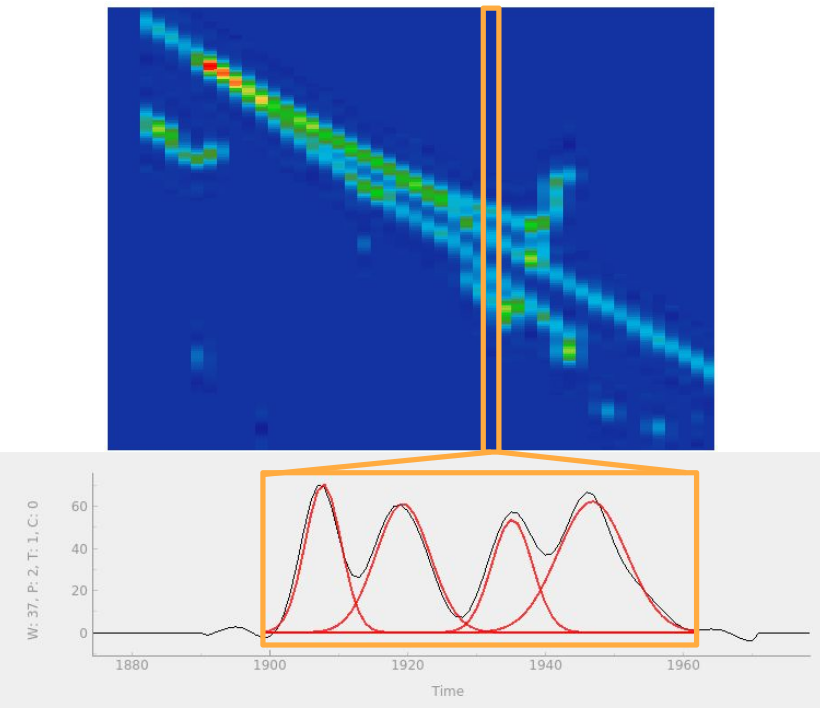
\includegraphics[width=0.55\textwidth]{gaushit}
\caption[gaushit]{
Event display of a simulated neutrino event, and a using the true ionisation charge (left), raw waveforms (middle) and deconvolved waveforms (right).
Fig. from Ref. \cite{EdPhD}.
}
\label{fig:gaushit}
\end{figure}

\subsection{Pandora Pattern Recognition}

%Pattern Recognition: Pandora
The output hits from the hit finding process are then used to perform 3D reconstruction, which is performed with the Pandora pattern recognition package\cite{pandora}. 
The package was first developed for the International Linear Collider, and later extended to other LArTPC experiments.
It is made up of over 100 individual algorithms, performing a specific task along the reconstruction chain.
The output from Pandora represents an interaction, containing a hierarchy of particles starting with a neutrino parent at the interaction vertex.
This reconstructed object is referred to as a \textit{slice}.  

The reconstruction begins with a workflow to reconstruct cosmic-like objects that leave long tracks inside the detector.
This workflow performs a 2D clustering on each wire plane independently, followed by 3D reconstruction under the assumption that all clusters are track-like.
Then, a cosmic rejection is performed to to identify if a cluster is cosmic-like or neutrino-like.
The cosmic removal at this stage is deliberately cautious such that only very unambiguous cosmic muons in nature are removed.

The remaining clusters are then input into a second workflow dedicated towards neutrino reconstruction.
This workflow begins with a slicing algorithm that divides the clusters into \textit{slices}, where each slice encapsulates hits coming from a single origin, representing an interaction.
Then, 2D clustering is re-performed on each wire plan independently, however, with a new assumption that clusters can be both track-like and shower-like.
A vertexing algorithm then identifies the interaction vertex of the slice and its associated clusters.
A series of pattern matching algorithms grows the interaction out of a neutrino vertex, and performs 3D reconstruction by matching 2D clusters across different planes.
The output 3D reconstructed object associated with a vertex ideally represent a \textit{particle} produced from an interaction.

At this stage, a track score is assigned to a particle if it has a track-like or a shower-like topology, which is determined by a dedicated Boosted Decision Tree (BDT).
The development work on the track and shower separation BDT and its importance not only in the reconstruction workflow but also in the analysis workflow will be covered in the next Sec. \ref{sec:trkshwbdt}.
Both track and shower reconstruction tools are then performed on the particle under the assumption if it is track-like or shower-like respectively. 
Finally, a hierarchy algorithm is performed to classify the hierarchy of particles in a slice, starting with a neutrino parent vertex, and other particles are children, grandchildren, etc. of the parent.

%Calorimetry reconstruction
The last stage of reconstruction is calorimetry computation for the output slices, and its associated particles.
Both track and shower calorimetry computations first convert ADC units to charge, or number of electrons, via multiplying a charge calibration constant.
The track calorimetry then computes the energy from charge using the Argoneut-parametrised ModBox recombination formalism, factoring in the electric distortion due the space charge effect.
Meanwhile, the shower calorimetry reconstruction converts the measured charge to energy by multiplying a shower calibration constant.
Once the SBND detector is operational, the calibration constants will be measured via dedicated calibration physics runs.
The charge calibration constant is expected to be computed from using a sample of anode to cathode crossing muon tracks while the shower calibration constant can be acquired from using standard candle of the neutral pion invariant mass \cite{}.

\subsection{Track-Shower Separation Boosted Decision Tree}
\label{sec:trkshwbdt}
As previously discussed, reconstructed particles from Pandora are assigned with a track score determined by Boosted Decision Tree (BDT), which is a binary classification machine learning tools.
The track score spans between 0 and 1 such that if a particle has a very high track score close to 1, then the particle is track-like.
Otherwise, if the track score is very close to 0, then the particle is shower-like.

The track-shower BDT has become more important in the reconstruction as well as the analysis workflow due to a new reconstruction paradigm introduced by Pandora.
The traditional reconstruction approach was to perform only either track or shower reconstruction on a particle based on its track score.
Meanwhile, the new paradigm performs both track and shower reconstruction on a particle regardless of the track score.
All reconstructed particles now have two sets of reconstruction variables for track-like and shower-like.
The analyzers have the freedom to decide which variables to use depending on their signal topology, and thus not pre-determined by Pandora.
The track score provides the necessary information if the signal topology is more track-like or shower-like and therefore, which appropriate reconstruction variables should be used for the analysis. 

The track-shower BDT was trained trained on series of reconstruction variables, has been recently updated to include new variables for the training.
The original BDT includes variables describing the geometrical topology of the particle such as its length, distance and direction with respect to the parent vertex, as well as calorimetry variables describing the charge distribution of the particle.
More details of the input variables and the training of the BDT can be found in Ref. \cite{EdPhD}.
The update extended beyond the original work to include a brand new set of variables describing how cone-like the charge distribution of a particle as well as a new set of variables describing the particle hierarchy.

The cone variables were first developed by the Pandora Warwick team \cite{}, which consist of three variables: (1) Halo total ratio, (2) concentration and (3) conicalness as depicted in Fig. \ref{fig:cone_variables}.
The diagrams depict hit distribution of a hypothetical particle, where each circle represents a hit associated with a charge value and the star represents the neutrino vertex.
The illustration is in 2D however the variables are computed in 3D.
The first variable is the halo-total ratio, illustrated in Fig. \ref{fig:halototalratio}.
The region outside of the Moliere radius, defined such that 90\% of the cluster energy is contained within this radius, is considered the halo region.
The halo hits are shown as green circles whereas hits inside the Moliere radius are shown as grey circles.
The halo-total ratio is then defined as 
\begin{equation}
	Halo\ Total\ Ratio = \frac{Charges\ in\ The\ Halo}{Total\ Charges}
\end{equation}
The second variable is called concentration, accounting for how concentrated the charge distribution to the centre of the cluster.
This is depicted in Fig. \ref{fig:concentration}, where each hit is assigned with a colour showing how weighted it is with respect to its orthogonal distance to the cluster direction.
The closer the hit to the centre, the more weighted it is.
The concentration variable is defined the total weighted charges divided by the total charge as following
\begin{equation}
	Concentration = \frac{\sum Charge \times Weight}{Total\ Charges}
\end{equation}
Finally, the conicalness variable examines the hit distribution at the end and the start of the cluster as depicted in Fig. \ref{fig:conicalness}. 
It is defined the ratio between the concentration at the end of the cluster compared to at the start of the cluster
\begin{equation}
	Conincalness = \frac{Concentration\ at\ The\ End}{Concentration\ at\ The\ Start}
\end{equation}
\begin{figure}[htbp!]
        \centering
        \begin{subfigure}[b]{0.329\textwidth}
            \centering
            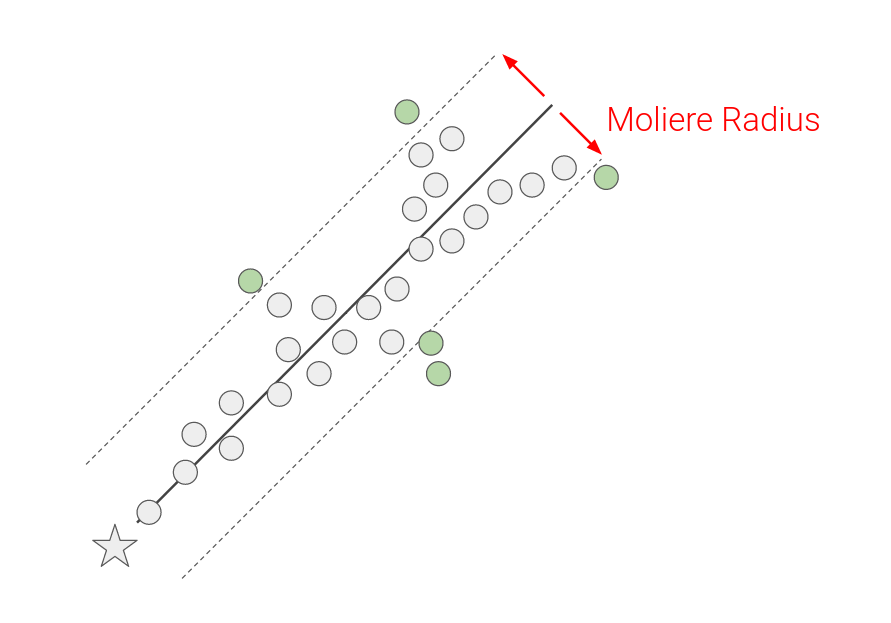
\includegraphics[width=\textwidth]{HaloTotalRatio}
            \caption{Halo Total Ratio}%
            \label{fig:halototalratio}
        \end{subfigure}
        \hfill
        \begin{subfigure}[b]{0.329\textwidth}  
            \centering 
            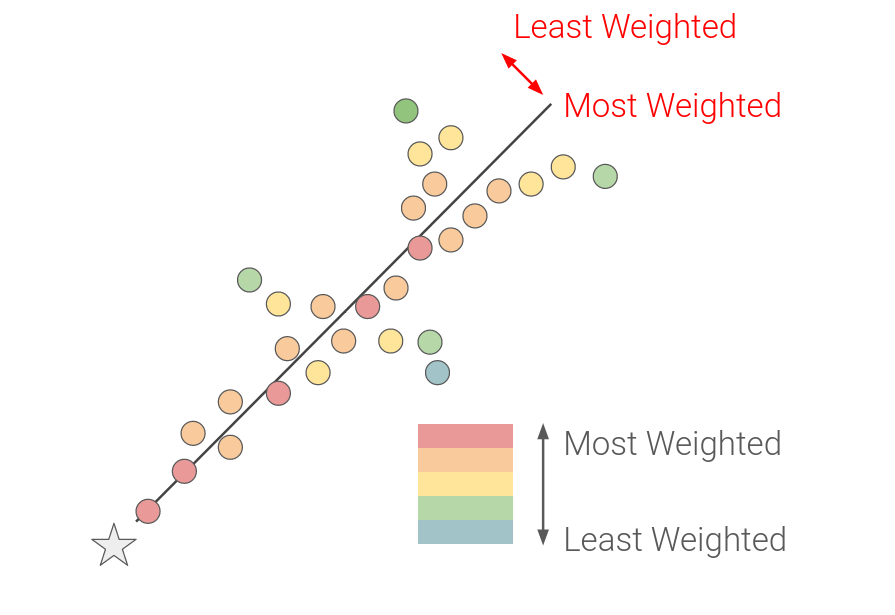
\includegraphics[width=\textwidth]{Concentration}
            \caption{Concentration}%
            \label{fig:concentration}
        \end{subfigure}
        \hfill
        \begin{subfigure}[b]{0.329\textwidth}  
            \centering 
            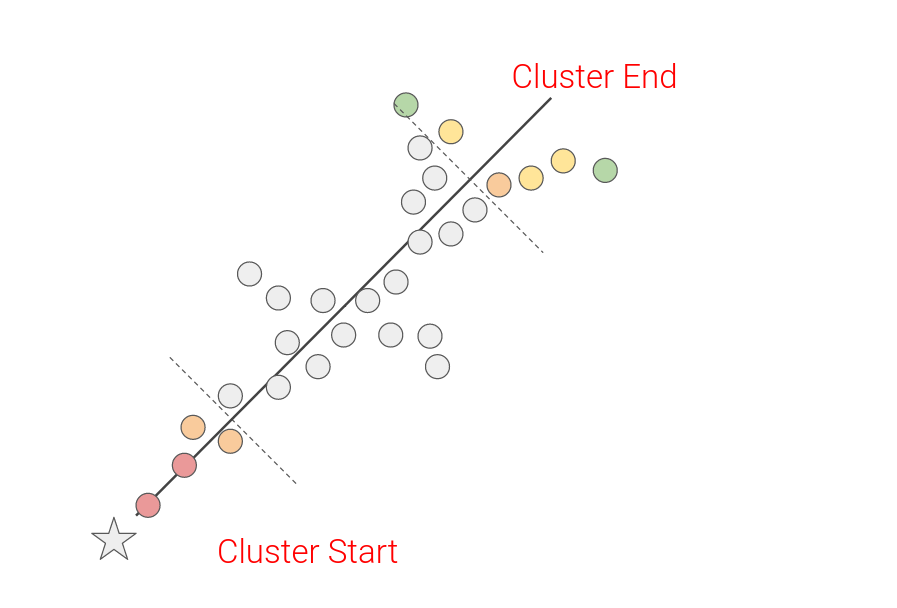
\includegraphics[width=\textwidth]{Conicalness}
            \caption{Conicalness}%
            \label{fig:conicalness}
        \end{subfigure}
        \caption[cone_variables]{
	Diagrams illustrating the variables describing how cone-like the charge distribution of a particle .
	}
        \label{fig:cone_variables}
\end{figure}

One new variable introduced to the track-shower separation BDT that describes the hierarchy of the particle within the reconstructed interaction or slice.
For a given particle, the daughters originating from that particle are identified and their number of hits are counted.
The distributions of the four new variables for a track-like and shower-like particle are shown in Fig. \ref{fig:bdt_features}.
The concentration and conicalness variables display the strongest separation power between tracks and showers compared to the halo total ratio and the number of daughter hits variables.

\begin{figure}[htbp!]
        \centering
        \begin{subfigure}[b]{0.45\textwidth}
            \centering
            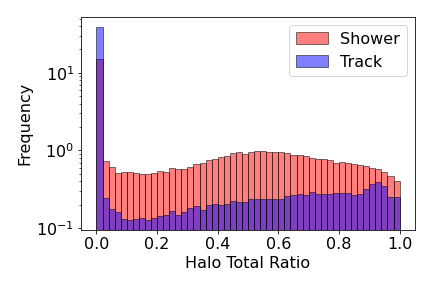
\includegraphics[width=\textwidth]{Feature_Halo_Total_Ratio}
            \caption{Halo Total Ratio}%
            \label{fig:feature_halototalratio}
        \end{subfigure}
        \hfill
        \begin{subfigure}[b]{0.45\textwidth}  
            \centering 
            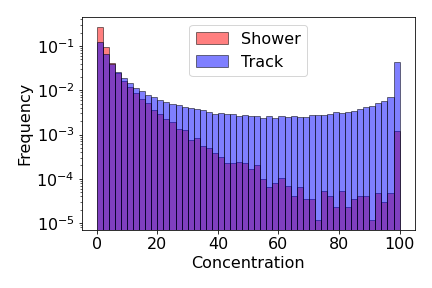
\includegraphics[width=\textwidth]{Feature_Concentration}
            \caption{Concentration}%
            \label{fig:feature_concentration}
        \end{subfigure}
        \hfill
        \begin{subfigure}[b]{0.45\textwidth}  
            \centering 
            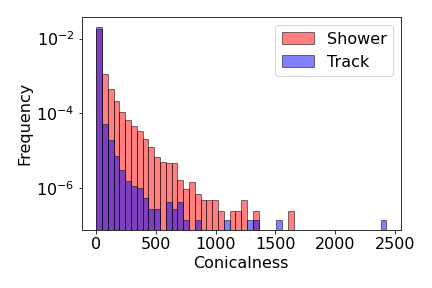
\includegraphics[width=\textwidth]{Feature_Conicalness}
            \caption{Conicalness}%
            \label{fig:feature_conicalness}
        \end{subfigure}
        \hfill
        \begin{subfigure}[b]{0.45\textwidth}  
            \centering 
            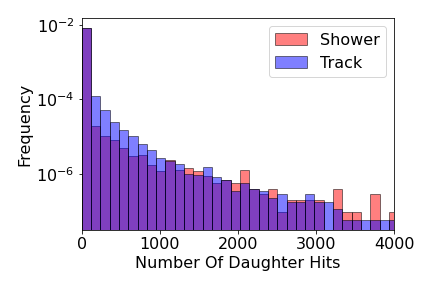
\includegraphics[width=\textwidth]{Feature_Number_Of_Daughter_Hits}
            \caption{Number of Daughter Hits}%
            \label{fig:feature_nDaughterHits}
        \end{subfigure}
        \caption[bdt_features]{
	Distributions of the new variables input into the track-shower separation BDT, plotted for track-like and shower-like particles.
	}
        \label{fig:bdt_features}
\end{figure}

Fig. \ref{fig:bdt_score} shows the score distribution of the BDT retrained with the four new variables.
The left figure shows two distinct distributions in red and blue for showers and tracks respectively.
This demonstrates a good separation power of the BDT, where particles with score less than 0.5 closely resemblance showers whilst particles with score more than 0.5 are more track-like.
The score distribution is broken down into different particle type as shown in the right figure.
The distribution is expected given that electrons and photons leave electromagnetic shower activities inside the detector whilst charged particles like muons, pions and protons leave track-like signatures. 
The updated BDT resulted in $0.1\sim2.0\%$ improvement in correctly classifies particle type as shower-like or track-like.
The track-shower separation score distribution will be used in downstream high level analysis tools, to be detailed in Sec. \ref{}, as well as will be employed as a cut variable in the HNL selection, to be detailed in Sec. \ref{}.

\begin{figure}[htbp!]
        \centering
        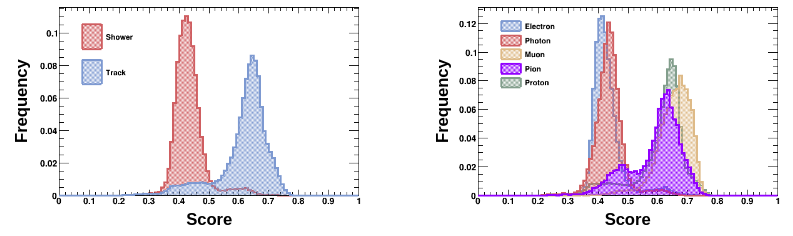
\includegraphics[width=\textwidth]{bdt_score}
        \caption[bdt_score]{
	Score distribution of the updated track-shower separation BDT, plotted for track-like and shower-like particles (left) and plotted for individual particle type (right).
	}
        \label{fig:bdt_score}
\end{figure}

\section{Reconstructing SBND: PDS and CRT Subsystems}
\label{sec:reco_others}

\subsection{PDS Reconstruction}

The reconstructions for the photodetectors, PMTs and X-ARAPUCAs, share the same steps of waveform deconvolution, hit finding and light reconstruction.
However, different algorithms and parameters settings are required for each photodetector type due to their difference in response.
More details on the PDS reconstruction at the SBND detector can be found in Ref. \cite{}.
The following focuses more on the reconstruction of PMTs which has an averaged Single Electron Response (SER) pulse peaking at $\sim 25$ ADC and a full width at half maximum of $\sim$ 10 ns.
The fast response of PMT plays the key role in the nanosecond timing resolution requirement for the HNL search.

Similarly to the signal processing in TPC reconstruction, the PMT waveform deconvolution also aims to remove noise and determine the waveform baseline.
Fig. \ref{fig:pds_reco_deconvolution} \cite{} depicts an example PMT waveform before and after the deconvolution.
The top figures shows the MC photons arrived at a given PMT in green.
The middle figure shows the simulated raw PMT waveform in blue, convolved with PMT response and noise.
The AC circuits of the PMTs lead to over/undershoots features across the waveform with respect to the baseline shown in red.
The waveform deconvolution step consists of a 1D deconvolution and an application of Gaussian filter to remove high frequency noise.
The resulting waveform is shown in orange in the bottom figure.
The bipolarity of the signals are fully removed while the integral and temporal position of the peaks are well-maintained.

\begin{figure}[tbp!]
        \centering
        \begin{subfigure}[b]{0.59\textwidth}
            \centering
            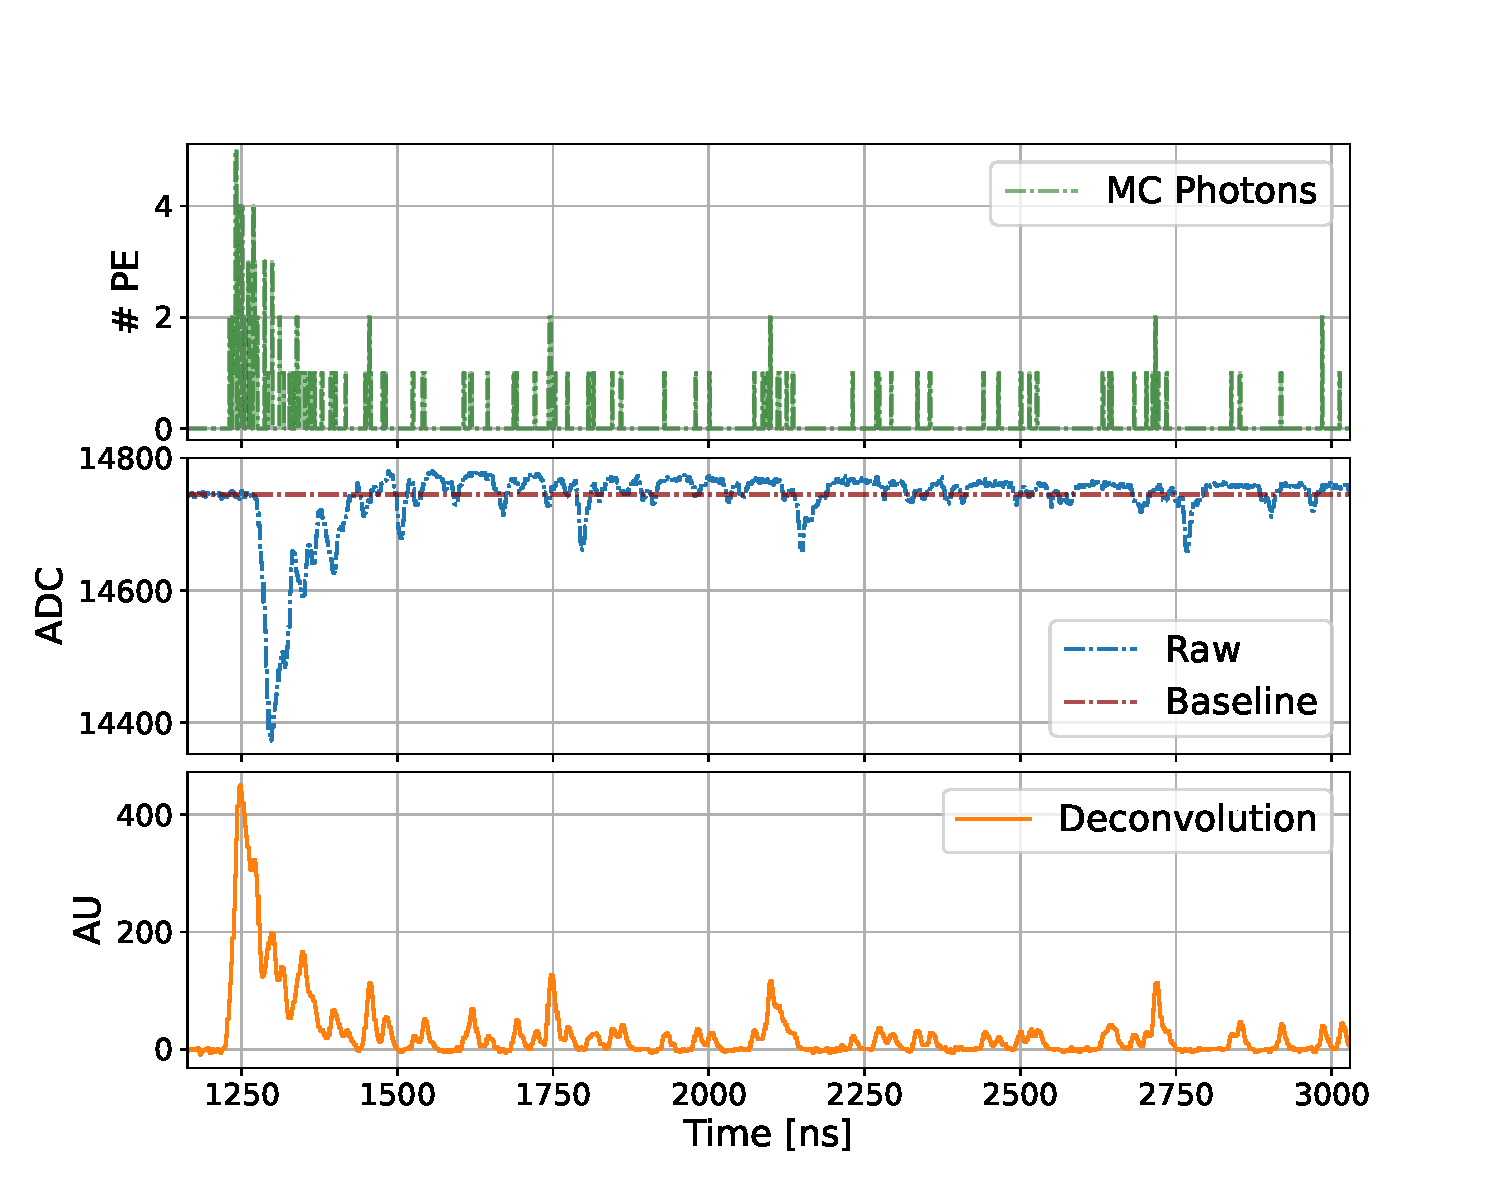
\includegraphics[width=\textwidth]{pds_reco_deconvolution}
            \caption{Waveform Deconvolution}
            \label{fig:pds_reco_deconvolution}
        \end{subfigure}
        \hfill
        \begin{subfigure}[b]{0.4\textwidth}  
            \centering 
            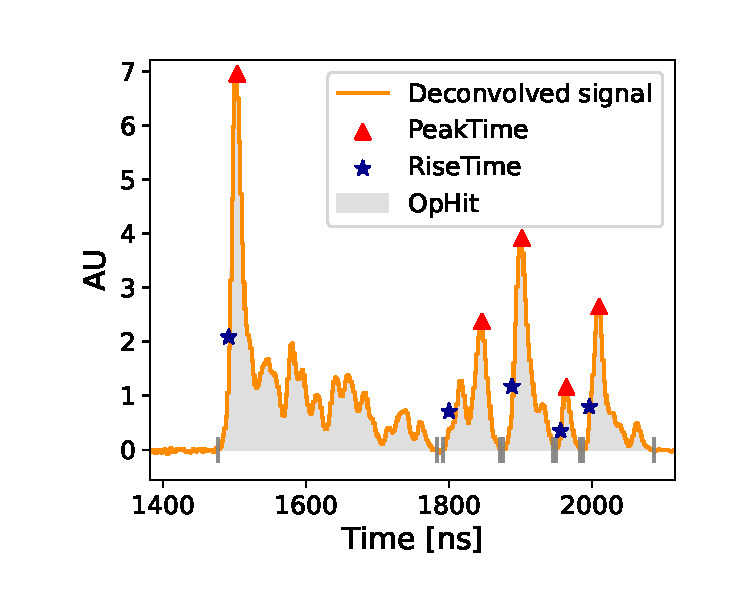
\includegraphics[width=\textwidth]{pds_reco_hit_finding}
            \caption{Hit Finding}
            \label{fig:pds_reco_hit_finding}
        \end{subfigure}
        \caption[pds_reco]{
	Both figures from Ref. \cite{}.
	}
        \label{fig:pds_reco}
\end{figure}

Then, the next step is to perform hit finding on the deconvolved PMT waveform as demonstrated in Fig. \ref{fig:pds_reco_hit_finding}.
The hit finding begins with a baseline subtraction, which is calculated using a 400 ns portion at the start and end of the deconvolved waveform, resulting in the waveform shown in orange.
Optical hits are identified by finding pulse goes above a threshold of $1/4$ the amplitude of the deconvolved SER and 3 standard deviations away from the baseline RMS.
The example shows 4 identified optical hits, with peak times denoted with red triangles.
The first optical hit contains multiple peaks merged into a single optical hit due to multiple photons arrive very closely to the PMT.
The rise time of an optical hit is then estimated as the time at which the pulse goes above 15\% of the peak  amplitude, denoted with blue stars, results in a resolution of 1.6 ns  in estimating the arrival time of the first photon contributing to the optical hit.
The integral of the optical hit are then computed to estimate the number of photoelectrons (PEs) of the hit.

After the hit finding, the light reconstruction algorithm then clusters optical hits into an \textit{optical flash}.
The length of an optical flash is set as 8 $\mu$s to account for the total light produced in an interaction, from both prompt and slow components of scintillation photons.
The clustering algorithm is based on several conditions on the calorimetry of the hits, timing distribution between hits and geometrical location of the PMTs.
The number of PEs in an optical flash is the sum of PEs of optical hits clustered in that flash, ideally represent the total light generated by an interaction. 

The start time of the optical flash represents the start time of an interaction, $t_0$, which is the key variable of the HNL search, and therefore requires great care in reconstruction.
The flash start time is the average of the rise time of optical hits in a flash for the PMTs that contribute 50\% of the prompt light in the 30 ns window of the largest PE pulse. 
Then, a correction is applied for the propagation of the photons from the scintillation position in the TPC to the PMTs, i.e. in the drift or $x$-direction.
This can done by exploiting the high density of PMTs as well as having PMTs sensitive to either or both direct and reflected light component.
As previously shown in Fig. \ref{fig:light_yield_Diego} with some discussions in Sec. \ref{sec:wls}, the arrival time distribution for the direct VUV and reflected visible photons varies with the drift distance.
For a given scintillation position, and therefore a drift position, the resulting amount of direct and visible photons can lead to a specific ratio of the two components seen by the PMTs.
And therefore, the ratio of the number of photons seen by TPB-coated PMTs to those seen by the uncoated PMTs can be used to compute the correction for the propagation effect.
The timing resolution of the flash time after propagation correction varies $\sim 2$ ns across the entire drfit distance, demonstrating the excellent capability of the PDS at SBND.

\subsection{Cosmic Ray Tagger Reconstruction}

The reconstruction workflow for the CRT subsystem is the simplest compared to the TPC and the PDS procedure.
As previously detailed, the output data of the CRT readouts are in group of 32 ADC values, for a single ADC per SiPM.
The reconstruction begins with a hit finding algorithm to identify which pair of SiPM in the group of 32 goes above a threshold.
The SiPM pair determines the lateral position of a cosmic muon hit within a CRT strip.
Then, a clustering algorithm groups hits from orthogonal CRT strips of the same wall within a 50 ns window to yield 3D space points.
For each CRT space point, the timing and calorimetry information is calculated and corrected for the propagation effect due to the longitudinal distance from the hit position to to the SiPM.
The final step of the reconstruction is to match space points from multiple CRT walls to form a CRT track.
Candidate tracks are evaluated from any combinations of space points from different taggers within a 100 ns coincidence window.
The best track candidate is selected by the goodness of timing agreement and prioritising three-point tracks over two-point tracks. 
The outputs of the CRT reconstruction are both CRT space points and CRT tracks. 

%********************************** %First Section  **************************************
\section{High Level Analysis Tools}

\subsection{Subsystems Matching}

\subsection{CRUMBS: Cosmic Rejection}

\subsection{Charge to Light Conversion}

\subsection{Particle Identification Tools}

\section{Concluding Remarks}
